% !TeX spellcheck = it_IT
\newpage
\section{Descrizione del dominio}
Un \textbf{concorso} è organizzato da uno o più \textbf{organizzatori}, che devono definire la durata del concorso in giorni, la scadenza per la sottomissione delle opere, la scadenza per la valutazione, il numero massimo di opere che possono essere presentate e la durata massima di ogni opera in minuti. Ogni concorso avrà dei \textbf{generi} consentiti (caratterizzati da un nome e descrizione), delle \textbf{lingue} accettate e dei criteri di partecipazione.\\

Ad ogni concorso un \textbf{regista} (che non può essere l'organizzatore) può presentare dei \textbf{cortometraggi} (fino al massimo indicato dagli organizzatori). Ogni cortometraggio è caratterizzato da un nome, la lingua, il genere, la durata in minuti e una trama.\\

Per ogni concorso gli organizzatori nominano dei \textbf{giudici} che compongono il comitato di valutazione. Ogni cortometraggio \textbf{partecipante} è assegnato a tre giudici, ognuno dei quali uno o più cortometraggi ma tutti di registi diversi. Ogni giudice può nominare un \textbf{giudice esterno} per ogni concorso per la valutazione di uno o più cortometraggi.\\

La valutazione avviene tramite una \textbf{recensione} scritta da un giudice relativamente ad una \textbf{partecipazione} di un cortometraggio, e contiene un punteggio da 0 a 5, un commento generale e una nota riservata.\\

Giudici, organizzatori e registi sono \textbf{utenti} del sistema con nome, cognome, codice fiscale ed email (usata per gli inviti dei giudici).

\newpage
\section{Schema concettuale}
\begin{center}
	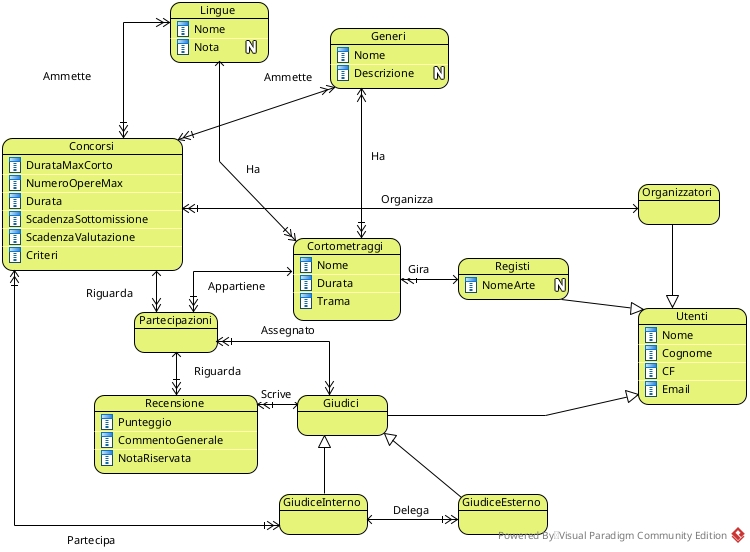
\includegraphics[scale=.5]{ERD_ConCorto.jpg}
\end{center}

\begin{note}
	Al momento della delega da parte di un \textbf{Giudice interno} di un \textbf{Giudice esterno}, quest'ultimo viene inserito nel database e viene assegnato alla valutazione di una determinata \textbf{partecipazione} scelta dal delegante.
\end{note}

\begin{note}
	Al momento dell'inserimento della \textbf{partecipazione} di un \textbf{cortometraggio} ad un \textbf{concorso}, vanno controllati i limiti imposti dall'\textbf{organizzatore} (\textit{DurataMaxCorto}, \textit{NumeroOpereMax}, lingue e generi accettati).
\end{note}

\subsection{Vincoli}
\subsubsection{Interrelazionali}
I vincoli interrelazionali sono:
\begin{itemize}
	\item Un giudice non può giudicare più di un cortometraggio per regista
	\item Un cortometraggio ha 3 giudici assegnati
	\item Un giudice può delegare al più un esterno per ogni concorso
	\item Un organizzatore non può partecipare come regista ad un concorso che organizza
	\item Un giudice può scrivere una sola recensione per cortometraggio per ogni concorso
	\item Se un giudice ha delegato la valutazione non può scrivere la recensione per il cortometraggio che ha delegato
\end{itemize}
\subsubsection{Intrarelazionali}
I vincoli intrarelazionali sono:
\begin{itemize}
	\item \textbf{Generi}: \textit{Descrizione} è NULLABLE
	\item \textbf{Lingue}: \textit{Nota} è NULLABLE
	\item \textbf{Concorsi}: \textit{DurataMaxCorto} $> 0$, \textit{NumeroOpereMax} $>0$, \textit{Durata} $>0$, \textit{ScadenzaSottomissione} $<$ \textit{ScadenzaValutazione}
	\item \textbf{Cortometraggi}: \textit{Durata} $>0$
	\item \textbf{Recensione}: $0\leq$\textit{Punteggio} $\leq 5$
	\item \textbf{Utenti}: \textit{Email} deve rispettare la seguente REGEX
	\begin{lstlisting}[language=Javascript]
		/^[\w-\.]+@([\w-]+\.)+[\w-]{2,4}$/g
	\end{lstlisting}
	\textit{CF} deve rispettare la seguente REGEX
	\begin{lstlisting}[language=Javascript]
		/^(?:[A-Z][AEIOU][AEIOUX]|[AEIOU]X{2}|[B-DF-HJ-NP-TV-Z]{2}[A-Z]){2}(?:[\dLMNP-V]{2}
		(?:[A-EHLMPR-T](?:[04LQ][1-9MNP-V]|[15MR][\dLMNP-V]|[26NS][0-8LMNP-U])|[DHPS]
		[37PT][0L]|[ACELMRT][37PT][01LM]|[AC-EHLMPR-T][26NS][9V])|(?:[02468LNQSU][048LQU]
		|[13579MPRTV][26NS])B[26NS][9V])(?:[A-MZ][1-9MNP-V][\dLMNP-V]{2}|[A-M][0L]
		(?:[1-9MNP-V][\dLMNP-V]|[0L][1-9MNP-V]))[A-Z]$/i
	\end{lstlisting}
	\item \textbf{Registi}: \textit{NomeArte} è NULLABLE
\end{itemize}
Dove non specificato, l'attributo è NON NULLABLE.

\newpage
\section{Schema logico relazionale}
\begin{center}
	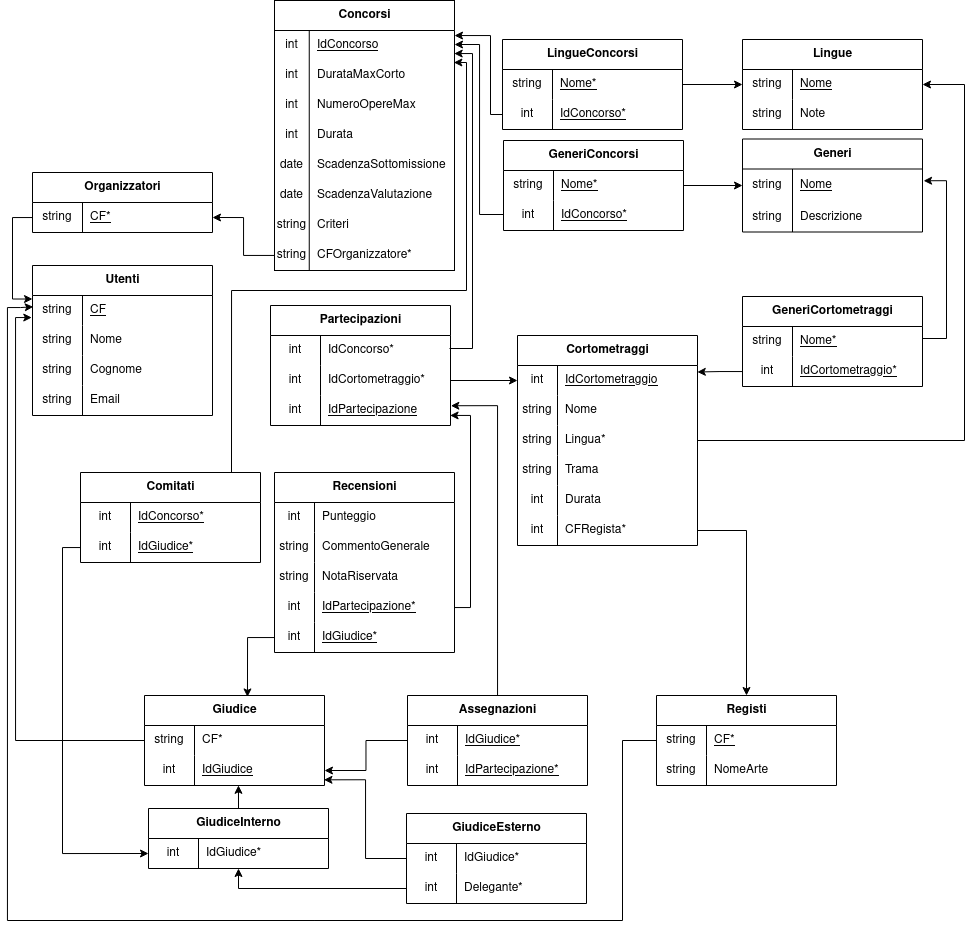
\includegraphics[scale=0.45]{BD0525_logico}
\end{center}

\subsection{Dipendenze funzionali}
Tutte le relazioni $R$ con attributi $A_1, \ldots, A_n$ chiave $K \notin A_1, \ldots, A_n$ hanno una sola dipendenza funzionale del tipo $K \to A_1, \ldots, A_n$.

\subsection{BCNF}
Tutte le relazioni sono in BCNF.

\newpage
\section{Interrogazioni in SQL}
Di seguito le sei interrogazioni richieste:
\begin{enumerate}
	\item[a.] Trova i nomi e le email degli utenti che sono registi e hanno diretto un cortometraggio di durata superiore a 25 minuti.
	\begin{lstlisting}[language=SQL]
		SELECT U.Nome, U.Email
		FROM Utenti U
		JOIN Registi R ON U.CF = R.CF
		JOIN Cortometraggi C ON R.CF = C.CFRegista
		WHERE C.Durata > 25;
	\end{lstlisting}
	\item[b.] Trova i concorsi con più di due lingue ammesse e con una durata massima inferiore a 120 giorni ordinati per numero di lingue in ordine decrescente.
	\begin{lstlisting}[language=SQL]
		SELECT C.IdConcorso, C.Durata, COUNT(L.Nome) AS NumeroLingue
		FROM Concorsi C
		JOIN LingueConcorsi LC ON C.IdConcorso = LC.IdConcorso
		JOIN Lingue L ON L.Nome = LC.Nome
		WHERE C.Durata < 120
		GROUP BY C.IdConcorso, C.Durata
		HAVING COUNT(L.Nome) > 2
		ORDER BY NumeroLingue DESC;
	\end{lstlisting} 
	\item[c.] Trova i generi di cortometraggi lunghi almeno 20 minuti che hanno una durata media superiore a 22 minuti, raggruppati per genere.
	\begin{lstlisting}[language=SQL]
		SELECT G.Nome, AVG(C.Durata) AS DurataMedia
		FROM GeneriCortometraggi GC
		JOIN Generi G ON G.Nome = GC.Nome
		JOIN Cortometraggi C ON C.IdCortometraggio = GC.IdCortometraggio
		WHERE C.Durata > 20
		GROUP BY G.Nome
		HAVING AVG(C.Durata) > 22;
	\end{lstlisting} 
	\item[d.] Trova i nomi dei cortometraggi che hanno almeno una recensione con punteggio superiore a 2.
	\begin{lstlisting}[language=SQL]
		SELECT C.Nome
		FROM Cortometraggi C
		WHERE EXISTS (
			SELECT *
			FROM Recensioni R
			JOIN Partecipazioni P ON R.IdPartecipazione = P.IdPartecipazione
			WHERE P.IdCortometraggio = C.IdCortometraggio AND R.Punteggio > 2
		);
	\end{lstlisting} 
	\item[e.] Trova i nomi dei concorsi in cui tutti i cortometraggi partecipanti hanno una durata inferiore a 30 minuti.
	\begin{lstlisting}[language=SQL]
		SELECT C.IdConcorso
		FROM Concorsi C
		WHERE NOT EXISTS (
		SELECT *
			FROM Partecipazioni P
			JOIN Cortometraggi CM ON P.IdCortometraggio = CM.IdCortometraggio
			WHERE P.IdConcorso = C.IdConcorso AND CM.Durata >= 30
		);
	\end{lstlisting}
	\newpage
	\item[f.] Trova i giudici che hanno assegnato un punteggio superiore alla media dei punteggi di tutti i giudici.
	\begin{lstlisting}[language=SQL]
		SELECT G.IdGiudice, G.CF
		FROM Giudici G
		WHERE EXISTS (
			SELECT *
			FROM Recensioni R
			WHERE R.IdGiudice = G.IdGiudice AND R.Punteggio > (
				SELECT AVG(Punteggio) 
				FROM Recensioni
			)
		);
	\end{lstlisting} 
\end{enumerate}

\newpage
\section{Piani di accesso}
\begin{enumerate}
	\item[I.] Piani di accesso \textbf{logico}
	\begin{figure}[!h]
		\centering
		\begin{minipage}{\textwidth}
			\centering
			
\includegraphics[scale=0.7]{1a.png}
			\captionof{figure}{Query \textit{a}}
		\end{minipage}
		\begin{minipage}{\textwidth}
			\centering
			
\includegraphics[scale=0.7]{1b.png}
			\captionof{figure}{Query \textit{b}}
		\end{minipage}
		\begin{minipage}{\textwidth}
			\centering
			
\includegraphics[scale=0.65]{1c.png}
			\captionof{figure}{Query \textit{c}}
		\end{minipage}
	\end{figure}
	
	\newpage
	\item[II.] Piani di accesso \textbf{fisico} senza uso di indici
	\begin{figure}[!h]
		\centering
		\begin{minipage}{\textwidth}
			\centering
			
\includegraphics[scale=0.7]{2a.png}
			\captionof{figure}{Query \textit{a}}
		\end{minipage}\\
		\begin{minipage}{\textwidth}
			\centering
			
\includegraphics[scale=0.7]{2b.png}
			\captionof{figure}{Query \textit{b}}
		\end{minipage}
	\end{figure}
	\begin{figure}[!h]
		\centering
		\begin{minipage}{\textwidth}
			\centering
			
\includegraphics[scale=0.55]{2c.png}
			\captionof{figure}{Query \textit{c}}
		\end{minipage}
	\end{figure}
	
	\newpage
	\item[III.] Piani di accesso \textbf{fisico} con uso di indici
	\begin{figure}[!h]
		\centering
		\begin{minipage}{\textwidth}
			\centering
			
\includegraphics[scale=0.7]{3a.png}
			\captionof{figure}{Query \textit{a}}
		\end{minipage}\\
	\end{figure}
	\begin{figure}[!h]
		\centering
		\begin{minipage}{\textwidth}
			\centering
			
\includegraphics[scale=0.7]{3b.png}
			\captionof{figure}{Query \textit{b}}
		\end{minipage} \hspace{50pt}
		\begin{minipage}{\textwidth}
			\centering
			
\includegraphics[scale=0.45]{3c.png}
			\captionof{figure}{Query \textit{c}}
		\end{minipage}
	\end{figure}
\end{enumerate}